%! Author = Josip Zeba
%! Date = 06/10/2022

% Preamble
\documentclass[a4paper,12pt,oneside,draft]{book}

% Packages
\usepackage{amsmath}
\usepackage{amssymb}
\usepackage{amsthm}
\usepackage[croatian]{babel}
\usepackage{tikz}
\usepackage{hyperref}
\usepackage{parskip}
\usepackage{titlesec}
\usepackage{setspace}
\usepackage{fancyhdr}
\usepackage{geometry}

% Povećanje razmaka između redaka
\onehalfspacing

% Zadavanje veličine korisne stranice i korekcija headheight
 \geometry{
 a4paper,
 total={150mm,237mm},
 left=30mm,
 top=30mm,
 }
\setlength{\headheight}{14.5pt}

% Promjena izgleda zaglavlja i podnožja
\pagestyle{fancy}
\renewcommand{\chaptermark}[1]{\markboth{\scshape{#1}}{}}
\renewcommand{\sectionmark}[1]{\markright{\itshape{#1}}{}}
\fancyhf{}
\rhead{\rightmark}
\lhead{\leftmark}
\cfoot{\thepage}

% Promjena izgleda poglavlja
\titleformat{\chapter}[display]
  {\scshape\Large}
  {\normalfont\filright{\chaptertitlename} \Huge\thechapter}
  {1ex}
  {\titlerule\vspace{1ex}\filright}
  [\vspace{1ex}\titlerule]

% Document
\begin{document}

% Naslovna strana
\begin{titlepage}

	\centering
	\scshape
	\vspace*{\baselineskip}

	%------------------------------------------------
	%	Naslov
	%------------------------------------------------

	\vspace{8\baselineskip}

	{\LARGE MATEMATIKA\\}

	\vspace{1\baselineskip}

	%------------------------------------------------
	%	Opis
	%------------------------------------------------

	Pripreme za državnu maturu iz matematike

	\vspace{8\baselineskip}

	%------------------------------------------------
	%	Autor
	%------------------------------------------------

	Autor

	{\scshape\Large Josip Zeba\\}

	\vfill

	%------------------------------------------------
	%	Mjesto i datum
	%------------------------------------------------

	\vspace{0.3\baselineskip}
	Zagreb

	2022.

\end{titlepage}

% Sadržaj
\setcounter{tocdepth}{1}
\clearpage
\ifpdf
	\phantomsection
\fi
\addcontentsline{toc}{chapter}{{\numberline{}\contentsname}}
\tableofcontents

% Poglavlja
\clearpage
\chapter{Realni brojevi}\label{ch:realni-brojevi}

\section{Računanje s realnim brojevima}\label{sec:računanje-s-realnim-brojevima}

Skup je bilo koja kolekcija različitih objekata u cjelini.

Elementi skupa mogu biti raznih vrsta: brojevi, ljudi, slova abecede, drugi skupovi itd.
Skupovi se dogovorno označavaju velikim slovima $A$, $B$, $C$, $\ldots$ te vitičastim zagradama $\{\ \}$ u koje se upisuju elementi.
Skupovi se mogu definirati, tj.\ opisati riječima ili eksplicitnim nabrajanjem svih elemenata između vitičastih zagrada.
Skup može biti konačan, beskonačan ili prazan.

Ako je nešto element nekog pojedinačnog skupa, odnosno pripada skupu, tada koristimo oznaku $\in$, a u slučaju da nije element skupa odnosno ne pripada skupu oznaku $\notin$.

Skupove možemo uspoređivati, pa ukoliko su svi elementi skupa $A$ i $B$ isti, možemo reći da je skup $A$ jednak skupu $B$, a tvrdnju zapisujemo $A = B$.
Nisu li svi elementi skupa $A$ i $B$ isti možemo zaključiti da je skup $A$ različit od skupa $B$, a tvrdnju zapisujemo $A \neq B$.

Ako je svaki član skupa $A$ također član skupa $B$, tada se za skup $A$ kaže da je podskup skupa $B$, a zapisuje se $A \subseteq B$.
Može se, također, zapisati $B \supseteq A$ odnosno skup $B$ je nadskup skupa $A$.
Ako je skup $A$ podskup i nije jednak skupu $B$, tada se za skup $A$ kaže da je pravi podskup skupa $B$, a zapisuje se $A \subset B$ ili možemo reći da je skup $B$ pravi nadskup skupa $A$ i zapisati $B \supset A$ kako prikazuje slika~\ref{fig:podskup}.

\begin{figure}
\begin{center}\vspace{0.25cm}
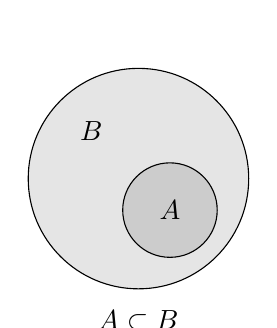
\begin{tikzpicture}[scale=0.8, every node/.style={scale=1}]
\filldraw[fill=gray!20,draw=black] (0,0) circle [radius=1.75];
\filldraw[fill=gray!40,draw=black] (0.5,-0.5) circle [radius=0.75];
\node at (0.5,-0.5) {$A$};
\node at (-0.75,0.75) {$B$};
\node at (0,-2.25) {$A \subset B$};
\end{tikzpicture}
\end{center}
\caption{Podskup}\label{fig:podskup}
\end{figure}

Postoji nekoliko načina za konstruiranje novih skupova od već postojećih.
Dva se skupa mogu \emph{zbrojiti} i to nazivamo unija skupova.
Unija skupova $A$ i $B$, označena sa $A \cup B$, je skup svih elemenata koji su članovi ili skupa $A$ ili skupa $B$.

Novi se skup također može konstruirati određivanjem \emph{zajedničkih} elemenata obaju skupova.
To nazivamo presjek skupova.
Presjek skupova $A$ i $B$, označen sa $A \cap B$, je skup svih elemenata koji su članovi i skupa $A$ i skupa $B$.

Jedna od operacija je i razlika skupova, odnosno \emph{oduzimanje} elemenata jednog skupa od drugoga.
Razlika skupova $A$ i $B$, označen sa $A \backslash B$, je skup koji čine svi članovi skupa $A$ koji nisu i u skupu $B$.
Slika~\ref{fig:operacije-sa-skupovima} prikazuje uniju, presjek i razliku skupova pomoću Vennovih dijagrama.

\begin{figure}[h!]
\begin{center}\vspace{0.25cm}
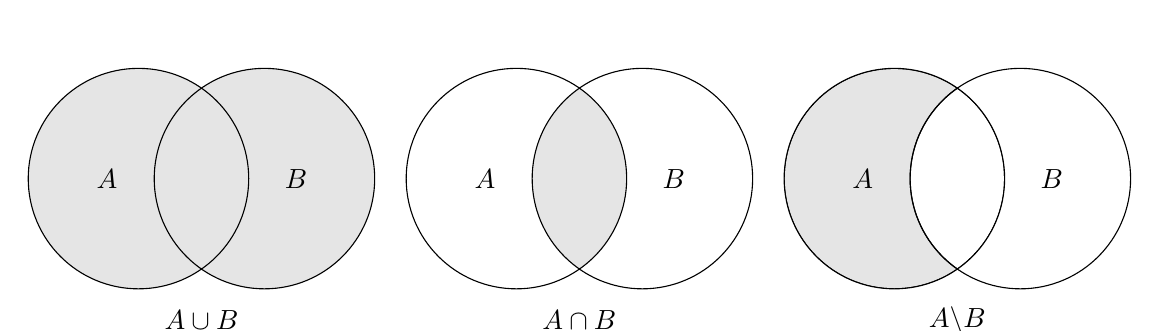
\begin{tikzpicture}[scale=0.8, every node/.style={scale=1}]
\filldraw[fill=gray!20,draw=black] (4,0) circle [radius=1.75] (6,0) circle [radius=1.75];
\node at (3.5,0) {$A$};
\node at (6.5,0) {$B$};
\node at (5,-2.25) {$A \cup B$};
\begin{scope}
  \clip (10,0) circle [radius=1.75];
  \fill[fill=gray!20] (12,0) circle [radius=1.75];
\end{scope}
\draw (10,0) circle [radius=1.75] (12,0) circle [radius=1.75];
\node at (9.5,0) {$A$};
\node at (12.5,0) {$B$};
\node at (11,-2.25) {$A \cap B$};
\begin{scope}
  \clip (16,0) circle [radius=1.75];
  \draw[fill=gray!20, even odd rule] (16,0) circle [radius=1.75] (18,0) circle [radius=1.75];
\end{scope}
\draw (16,0) circle [radius=1.75] (18,0) circle [radius=1.75];
\node at (15.5,0) {$A$};
\node at (18.5,0) {$B$};
\node at (17,-2.25) {$A \backslash B$};
\end{tikzpicture}
\end{center}
\caption{Operacije sa skupovima}\label{fig:operacije-sa-skupovima}
\end{figure}

\subsection{Skup prirodnih brojeva}\label{subsec:skup-prirodnih-brojeva}
Skup prirodnih brojeva označavamo s oznakom $\mathbb{N}$.
Ovaj skup je zatvoren s obzirom na zbrajanje i množenje.
\[ \mathbb{N}=\{1,2,3,4,5,\ldots\}. \]
Skup se često proširuje brojem 0 te ga u tom slučaju označavamo s $\mathbb{N}_0$.
Kažemo da je prirodni broj $n$ djeljiv s prirodnim brojem $m$ ako postoji $k \in \mathbb{N}$ sa svojstvom da je $n=k \cdot m$.
Tada je $n$ višekratnik broja $m$ te je $m$ djelitelj broja $n$ ili kraće $m|n$.

U skupu prirodnih brojeva svaki broj ima svog neposrednog sljedbenika ($n+1$), a samim time, osim broja 1, i svog neposrednog prethodnika ($n-1$).

Najveći zajednički djelitelj prirodnih brojeva $a$, $b$ i $c$ je najveći broj koji dijeli sve te brojeve i označavamo ga nzd ($a$, $b$, $c$), a najmanji zajednički višekratnik prirodnih brojeva $a$, $b$ i $c$ je najmanji prirodni broj koji je djeljiv sa svakim od tih brojeva i označavamo ga nzv ($a$, $b$ i $c$).

Prirodan broj veći od 1 je prost broj ako je djeljiv samo s 1 i sa samim sobom.
Broj je složen ako nije prost, s iznimkom broja 1 koji ne držimo ni prostim ni složenim.
Svaki se prirodan broj može napisati u obliku umnoška prostih brojeva.

Kriteriji djeljivosti prirodnih brojeva s brojevima od 0 do 10 su:
\begin{itemize}
  \item broj je djeljiv s 2 ako mu je zadnja znamenka 0, 2, 4, 6, 8, odnosno paran broj,
  \item broj je djeljiv s 3 ako mu je zbroj znamenaka djeljiv s 3,
  \item broj je djeljiv sa 4 ako mu je dvoznamenkasti završetak djeljiv s 4,
  \item broj je djeljiv s 5 ako mu je zadnja znamenka 0 ili 5,
  \item broj je djeljiv sa 6 ako je djeljiv i s 2 i s 3,
  \item broj je djeljiv sa 7 ako je razlika između broja koji se dobije micanjem broja jedinice i dvostruke znamenke jedinica toga broja djeljiva sa 7,
  \item broj je djeljiv s 8 ako mu je troznamenkasti završetak djeljiv s 8,
  \item broj je djeljiv s 9 ako mu je zbroj znamenaka djeljiv s 9,
  \item broj je djeljiv s 10 ako mu je zadnja znamenka 0.
\end{itemize}

\subsection{Skup cijelih brojeva}\label{subsec:skup-cijelih-brojeva}
Skup cijelih brojeva označavamo s oznakom $\mathbb{Z}$.
Potreba za ovim skupom dolazi iz razloga kako rezultat oduzimanja prirodnih brojeva nije uvijek prirodan broj, stoga se skup prirodnih brojeva proširuje s 0 i negativnim cijelim brojevima.
Skup je zatvoren s obzirom na zbrajanje, oduzimanje i množenje.
\[ \mathbb{Z}=\{\ldots,-3,-2,-1,0,1,2,3,\ldots\}. \]
Za svaki cijeli broj $a \neq 0$ postoji cijeli broj $-a$ tako da vrijedi da je njihov zbroj jednak 0.
Broj $-a$ je suprotni broj broja $a$.

Dijeljenje s nulom nije definirano.

\subsection{Skup racionalnih brojeva}\label{subsec:skup-racionalnih-brojeva}
Skup racionalnih brojeva označavamo s oznakom $\mathbb{Q}$.
Činjenica da količnik dvaju cijelih brojeva općenito nije cijeli broj nameće potrebu za proširenjem skupa cijelih brojeva.
Skup racionalnih brojeva zatvoren je s obzirom na zbrajanje, oduzimanje, množenje i dijeljenje.
\[ \mathbb{Q}=\left\{\frac{a}{b} : a,b \in \mathbb{Z}, b \neq 0 \right\}. \]
Svaki je racionalni broj je moguće zapisati u obliku razlomka, gdje je broj $a$ brojnik, a broj $b$ nazivnik razlomka.
Svaki racionalan broj ima konačan ili beskonačan periodičan decimalni prikaz.
Provedemo li razlomkom zadano dijeljenje cijelih brojeva, dobit ćemo racionalan broj zapisan u decimalnom obliku.

Za svaki racionalni broj $\displaystyle \frac{a}{b}$ i svaki broj $m$ različiti od nule vrijedi
\[ \frac{a}{b} = \frac{a \cdot m}{b \cdot m}, \]
pri čemu, ako jednakost čitamo s lijeva na desno, govorimo o proširivanju razlomka, a u suprotnom smjeru, govorimo o skraćivanju razlomka.

Pravi razlomak je razlomak kojem je brojnik manji od nazivnika.
Kada govorimo o zbroju prirodnog broja $n$ i razlomka, govorimo o mješovitom broju
\[ n + \frac{a}{b} = n\frac{a}{b}, \]
Zbrajanje i oduzimanje razlomaka provodi se na način da se razlomci svedu, odnosno prošire na zajednički nazivnik te se njihovi brojnici zbroje, odnosno oduzmu.

Množenje dvaju razlomaka provodi se na način da se pomnože brojnik s brojnikom i nazivnik s nazivnikom te se dijeljenje razlomaka zamjenjuje s množenjem na način da djelitelja zapišemo u recipročnom obliku, odnosno zamijenimo mjesta brojniku i nazivniku te nakon toga provedemo množenje dvaju razlomaka.

\subsection{Skup iracionalnih brojeva}\label{subsec:skup-iracionalnih-brojeva}
Postoje brojevi koji nisu racionalni, koje nije moguće predočiti kao količnik dvaju cijelih brojeva, odnosno zapisati u obliku razlomka.
Takvi se brojevi zovu iracionalni brojevi.
Skup iracionalnih brojeva označavamo s oznakom $\mathbb{I}$.
Brojevi $\sqrt{2}$, $\sqrt{3}$, $\pi$ i $e$  primjeri su nekih iracionalnih brojeva.

\subsection{Skup realnih brojeva}\label{subsec:skup-realnih-brojeva}
Skup realnih brojeva označavamo s oznakom $\mathbb{R}$ i sastoji se od skupa racionalnih i iracionalnih brojeva.
Skup realnih brojeva zatvoren je s obzirom na zbrajanje, oduzimanje, množenje i dijeljenje.
\[ \mathbb{R}=\mathbb{Q} \cup \mathbb{I}. \]
Svaki realni broj $a$ možemo prikazati u konačnom ili beskonačnom decimalnom zapisu.
Također možemo reći da vrijedi da je svaki prirodan broj ujedno i cijeli broj, a svaki cijeli ujedno i racionalni te svaki racionalni ujedno i realni broj pa vrijedi da je
\[ \mathbb{N} \subset \mathbb{Z} \subset \mathbb{Q} \subset \mathbb{R}. \]
Aksiomi polja skupa realnih brojeva su:
\begin{itemize}
  \item komutativnost: $a+b=b+a, \quad a \cdot b = b \cdot a$,
  \item asocijativnost: $(a+b)+c=a+(b+c), \quad (a \cdot b) \cdot c = a \cdot (b \cdot c)$,
  \item distributivnost: $a \cdot (b + c) = a \cdot b + a \cdot c$,
  \item neutralni elementi, 0 za zbrajanje i 1 za množenje: $a + 0 = a, \quad a \cdot 1 = a$
  \item suprotni i inverzni broj: $\displaystyle a + (-a) = 0, \quad a \cdot \frac{1}{a} = 1 \quad a \neq 0.$
\end{itemize}

\section{Brojevni pravac i intervali}\label{sec:brojevni-pravac-i-intervali}
Brojevni pravac je pravac na kojem je svakomu realnom broju pridružena jedna jedina točka.
Brojevni pravac služi za predočavanje brojeva i grafičko računanje njima.
Slika~\ref{fig:brojevni-pravac} prikazuje brojevni pravac.

\begin{figure}[h!]
\begin{center}\vspace{0.25cm}
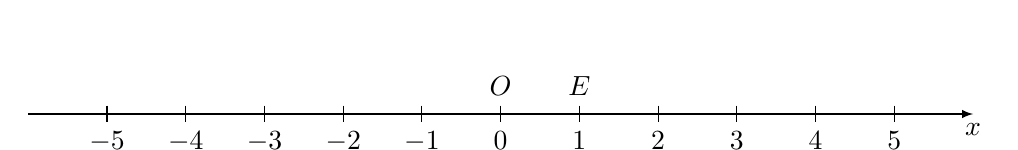
\begin{tikzpicture}
\draw[-latex] (-6,0) -- (6,0) coordinate[label=below: $x$] (x);
\foreach \x in  {-5,-4,-3,-2,-1,0,1,2,3,4,5}
\draw[shift={(\x,0)},color=black] (0pt,3pt) -- (0pt,-3pt);
\foreach \x in {-5,-4,-3,-2,-1,0,1,2,3,4,5}
\draw[shift={(\x,0)},color=black] (0pt,-3pt) node[below] {$\x$};
\draw (0cm,3pt) node[above] {$O$};
\draw (1cm,3pt) node[above] {$E$};
\end{tikzpicture}
\end{center}
\caption{Brojevni pravac}\label{fig:brojevni-pravac}
\end{figure}

Na pravcu se najprije odabere točka $O$ odnosno ishodište, koja predstavlja 0, a zatim jedinična točka 1 s oznakom $E$.
Dužina $\overline{OE}$ predstavlja jediničnu duljinu.
Točkama na desnoj strani od $O$ odgovaraju pozitivni realni brojevi, odnosno veći brojevi, a na lijevoj strani negativni, odnosno manji brojevi od promatranoga.
Bilo kojem realnom broju $a$ odgovara točka $A$, tako da je dužina $\overline{OA}$ (mjerena jediničnom duljinom) jednaka $a$ jediničnih duljina.
Između bilo koja dva realna broja postoji beskonačno mnogo racionalnih i iracionalnih brojeva.

Skup svih realnih brojeva $x$ za koje vrijedi $a<x<b$ gdje su $a$ i $b$ također realni brojevi, zovemo intervalom i zapisujemo $\langle a,b \rangle$.
Intervali mogu biti poluzatvoreni $[a,b \rangle$, ako je $a \leq x<b$, poluotvoreni $\langle a,b]$, ako je $a<x \leq b$ ili zatvoreni $[a,b]$, ako je $a \leq x \leq b$, kako je prikazano na slici~\ref{fig:intervali}

\begin{figure}[h!]
\begin{center}\vspace{0.5cm}
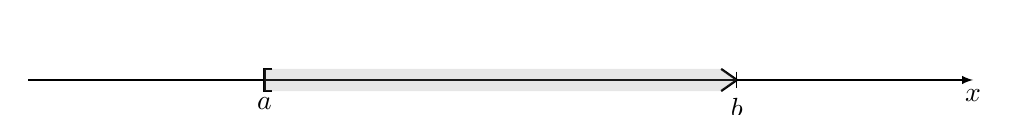
\begin{tikzpicture}
\draw[-latex] (-6,0) -- (6,0) coordinate[label=below: $x$] (x);
\foreach \x in  {-3,3}
\draw[shift={(\x,0)},color=black] (0pt,3pt) -- (0pt,-3pt);
\draw (-3cm,-3pt) node[below] {$a$};
\draw (3cm,-3pt) node[below] {$b$};
\draw[thick] (-2.9,4pt) -- (-3,4pt) -- (-3,-4pt) -- (-2.9,-4pt);
\draw[thick] (2.8,-4pt) -- (3,0) -- (2.8,4pt);
\fill[opacity = 0.2, gray] (-3,-4pt) -- (2.8, -4pt) -- (3, 0) -- (2.8, 4pt) -- (-3,4pt);
\end{tikzpicture}

\vspace{0.5cm}
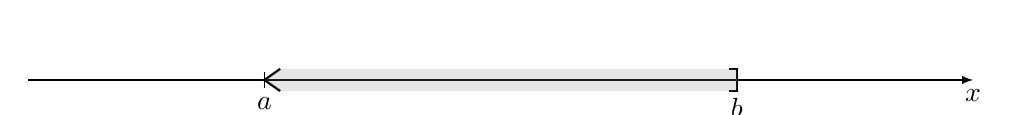
\begin{tikzpicture}
\draw[-latex] (-6,0) -- (6,0) coordinate[label=below: $x$] (x);
\foreach \x in  {-3,3}
\draw[shift={(\x,0)},color=black] (0pt,3pt) -- (0pt,-3pt);
\draw (-3cm,-3pt) node[below] {$a$};
\draw (3cm,-3pt) node[below] {$b$};
\draw[thick] (2.9,4pt) -- (3,4pt) -- (3,-4pt) -- (2.9,-4pt);
\draw[thick] (-2.8,-4pt) -- (-3,0) -- (-2.8,4pt);
\fill[opacity = 0.2, gray] (3,-4pt) -- (-2.8, -4pt) -- (-3, 0) -- (-2.8, 4pt) -- (3,4pt);
\end{tikzpicture}

\vspace{0.5cm}
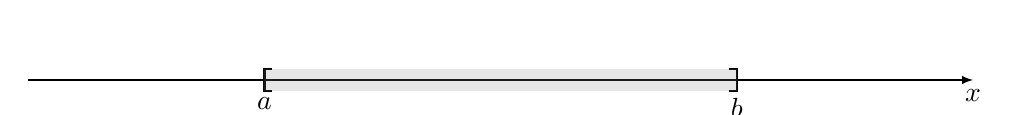
\begin{tikzpicture}
\draw[-latex] (-6,0) -- (6,0) coordinate[label=below: $x$] (x);
\foreach \x in  {-3,3}
\draw[shift={(\x,0)},color=black] (0pt,3pt) -- (0pt,-3pt);
\draw (-3cm,-3pt) node[below] {$a$};
\draw (3cm,-3pt) node[below] {$b$};
\draw[thick] (2.9,4pt) -- (3,4pt) -- (3,-4pt) -- (2.9,-4pt);
\draw[thick] (-2.9,4pt) -- (-3,4pt) -- (-3,-4pt) -- (-2.9,-4pt);
\fill[opacity = 0.2, gray] (3,-4pt) -- (-3, -4pt) -- (-3, 4pt) -- (3,4pt);
\end{tikzpicture}
\end{center}
\caption{Intervali}\label{fig:intervali}
\end{figure}

Neke granice intervala mogu biti i beskonačne pa tako skup svih realnih brojeva za koje vrijedi $x>a$ možemo zapisati u obliku intervala $\langle a,+\infty \rangle$, a skup svih realnih brojeva za koje vrijedi $x<a$ možemo zapisati u obliku intervala $\langle -\infty , a \rangle$, kako je prikazano na slici~\ref{fig:beskonačni-intervali}.

\begin{figure}[h!]
\begin{center}\vspace{0.5cm}
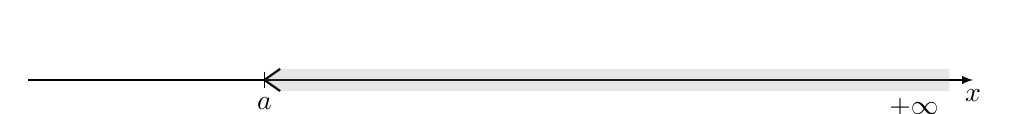
\begin{tikzpicture}
\draw[-latex] (-6,0) -- (6,0) coordinate[label=below: $x$] (x);
\foreach \x in  {-3}
\draw[shift={(\x,0)},color=black] (0pt,3pt) -- (0pt,-3pt);
\draw (-3cm,-3pt) node[below] {$a$};
\draw (5.25,-3pt) node[below] {$+\infty$};
\draw[thick] (-2.8,4pt) -- (-3,0pt) -- (-2.8,-4pt);
\fill[opacity = 0.2, gray] (-2.8,-4pt) -- (5.7, -4pt) -- (5.7, 4pt) -- (-2.8, 4pt) -- (-3,0pt);
\end{tikzpicture}

\vspace{0.5cm}
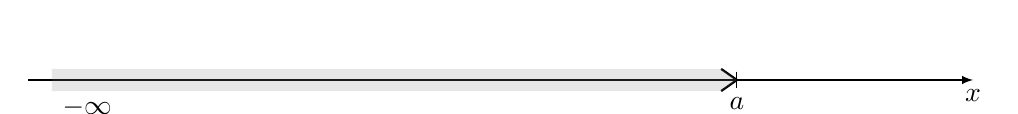
\begin{tikzpicture}
\draw[-latex] (-6,0) -- (6,0) coordinate[label=below: $x$] (x);
\foreach \x in  {3}
\draw[shift={(\x,0)},color=black] (0pt,3pt) -- (0pt,-3pt);
\draw (3cm,-3pt) node[below] {$a$};
\draw (-5.25,-3pt) node[below] {$-\infty$};
\draw[thick] (2.8,4pt) -- (3,0pt) -- (2.8,-4pt);
\fill[opacity = 0.2, gray] (2.8,-4pt) -- (-5.7, -4pt) -- (-5.7, 4pt) -- (2.8, 4pt) -- (3,0pt);
\end{tikzpicture}
\end{center}
\caption{Beskonačni intervali}\label{fig:beskonačni-intervali}
\end{figure}


% Popis literature
\bibliography{main}
\bibliographystyle{plain}

\end{document}